% Latex template: mahmoud.s.fahmy@students.kasralainy.edu.eg
% For more details: https://www.sharelatex.com/learn/Beamer

\documentclass{beamer}					% Document class

\setbeamertemplate{footline}[text line]{%
  \parbox{\linewidth}{\vspace*{-8pt}Statistical Methods For Stochastic Biological Systems\hfill\insertshortauthor\hfill\insertpagenumber}}
\setbeamertemplate{navigation symbols}{}

\usepackage[english]{babel}				% Set language
\usepackage[utf8x]{inputenc}			% Set encoding

\mode<presentation>						% Set options
{
  \usetheme{default}					% Set theme
  \usecolortheme{default} 				% Set colors
  \usefonttheme{default}  				% Set font theme
  \setbeamertemplate{caption}[numbered]	% Set caption to be numbered
}

% Uncomment this to have the outline at the beginning of each section highlighted.
%\AtBeginSection[]
%{
%  \begin{frame}{Outline}
%    \tableofcontents[currentsection]
%  \end{frame}
%}

\usepackage{graphicx}					% For including figures
\usepackage{booktabs}					% For table rules
\usepackage{hyperref}					% For cross-referencing

\title{Deep generative models for biologists}	% Presentation title
\author{Clayton W. Seitz}								% Presentation author
\date{\today}									% Today's date	

\begin{document}

% Title page
% This page includes the informations defined earlier including title, author/s, affiliation/s and the date
\begin{frame}
  \titlepage
\end{frame}

% Outline
% This page includes the outline (Table of content) of the presentation. All sections and subsections will appear in the outline by default.
\begin{frame}{Outline}
  \tableofcontents
\end{frame}

% The following is the most frequently used slide types in beamer
% The slide structure is as follows:
%
%\begin{frame}{<slide-title>}
%	<content>
%\end{frame}


\section{Deep Generative Models}

\begin{frame}{Discriminative and generative models}

Say we have a set of variables $\mathbf{x} = (x_{1},x_{2},...,x_{n})$ which might have some statistical dependence\\
\vspace{0.2in}
In supervised \textcolor{red}{discriminative} learning, we may use observations of $\mathbf{x}$ to try and learn distributions such as $p(x_{2}|x_{1})$ (i.e., inference)\\
\vspace{0.2in}
The variable $\mathbf{x}$ might be an amino acid sequence, DNA sequence, microscopy image, etc.\\
\vspace{0.2in}
In supervised \textcolor{red}{generative} learning, we try to explicity learn the joint distribution $p(\mathbf{x})=p(x_{1}|x_{2},...,x_{n})p(x_{2}|x_{3},...,x_{n}),...,p(x_{n})$, which is generally more difficult. 

\end{frame}

\begin{frame}{The basic sampling problem}

Suppose we are given a joint distribution

\begin{equation*}
p(\mathbf{x}) = \frac{1}{Z}\tilde{p}(\mathbf{x})
\end{equation*}

where $p(\mathbf{x})$ is easy to compute but $Z$ is (too) hard to compute.\\
\vspace{0.1in}
This \textcolor{red}{very important} situation arises in several contexts:\\
\vspace{0.1in}
1. In \textcolor{red}{Bayesian models} where $p(x_{1},x_{2}) := p(x_{1}|x_{2})p(x_{2})$ is easy to compute but
$Z = \int p(x_{1}|x_{2})p(x_{2})dx_{2}$ can be very difficult or impossible to
compute.\\
\vspace{0.1in}
2. In models from statistical physics, e.g. the Ising model, we only know
$p(\mathbf{x}) = e^{−H(\mathbf{x})}$ where $H(\mathbf{x})$ is the Hamiltonian
- the Ising model is an example of a \textcolor{red}{Markov network} or an \textcolor{red}{undirected graphical model}.

\end{frame}

\begin{frame}{Approximating the joint distribution}

Suppose we are given a joint distribution

\begin{equation*}
p(\mathbf{x}) = \frac{1}{Z}\tilde{p}(\mathbf{x})
\end{equation*}
 
\textcolor{red}{Variational methods} are generally useful for Bayesian inference like $p(x_{1}|x_{2})$ but can also be used to evaluate $p(\mathbf{x})$ by autoencoding $\mathbf{x}$ (called a variational autoencoder)\\
\vspace{0.1in}
\textcolor{red}{Generative adversarial networks (GANs)} model $p(\mathbf{x})$ directly\\
\vspace{0.1in}
In special scenarios, we may know $\tilde{p}(\mathbf{x})$ and we can use \textcolor{red}{Monte-Carlo Markov Chain (MCMC)} methods

\end{frame}

\begin{frame}{Applying generative models to biological data}
\begin{figure}
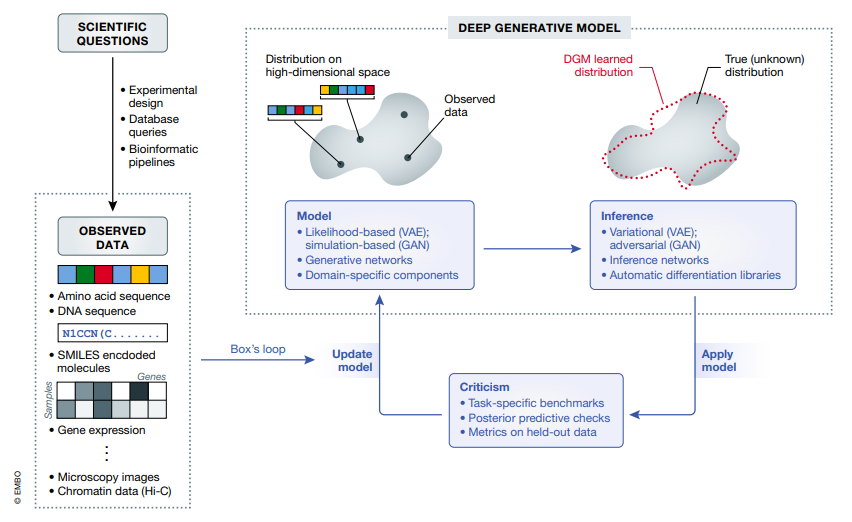
\includegraphics[height=65mm, width=105mm]{dbm}
\end{figure}
\end{frame}

\begin{frame}{Generative models: variational autoencoder}

\begin{center}
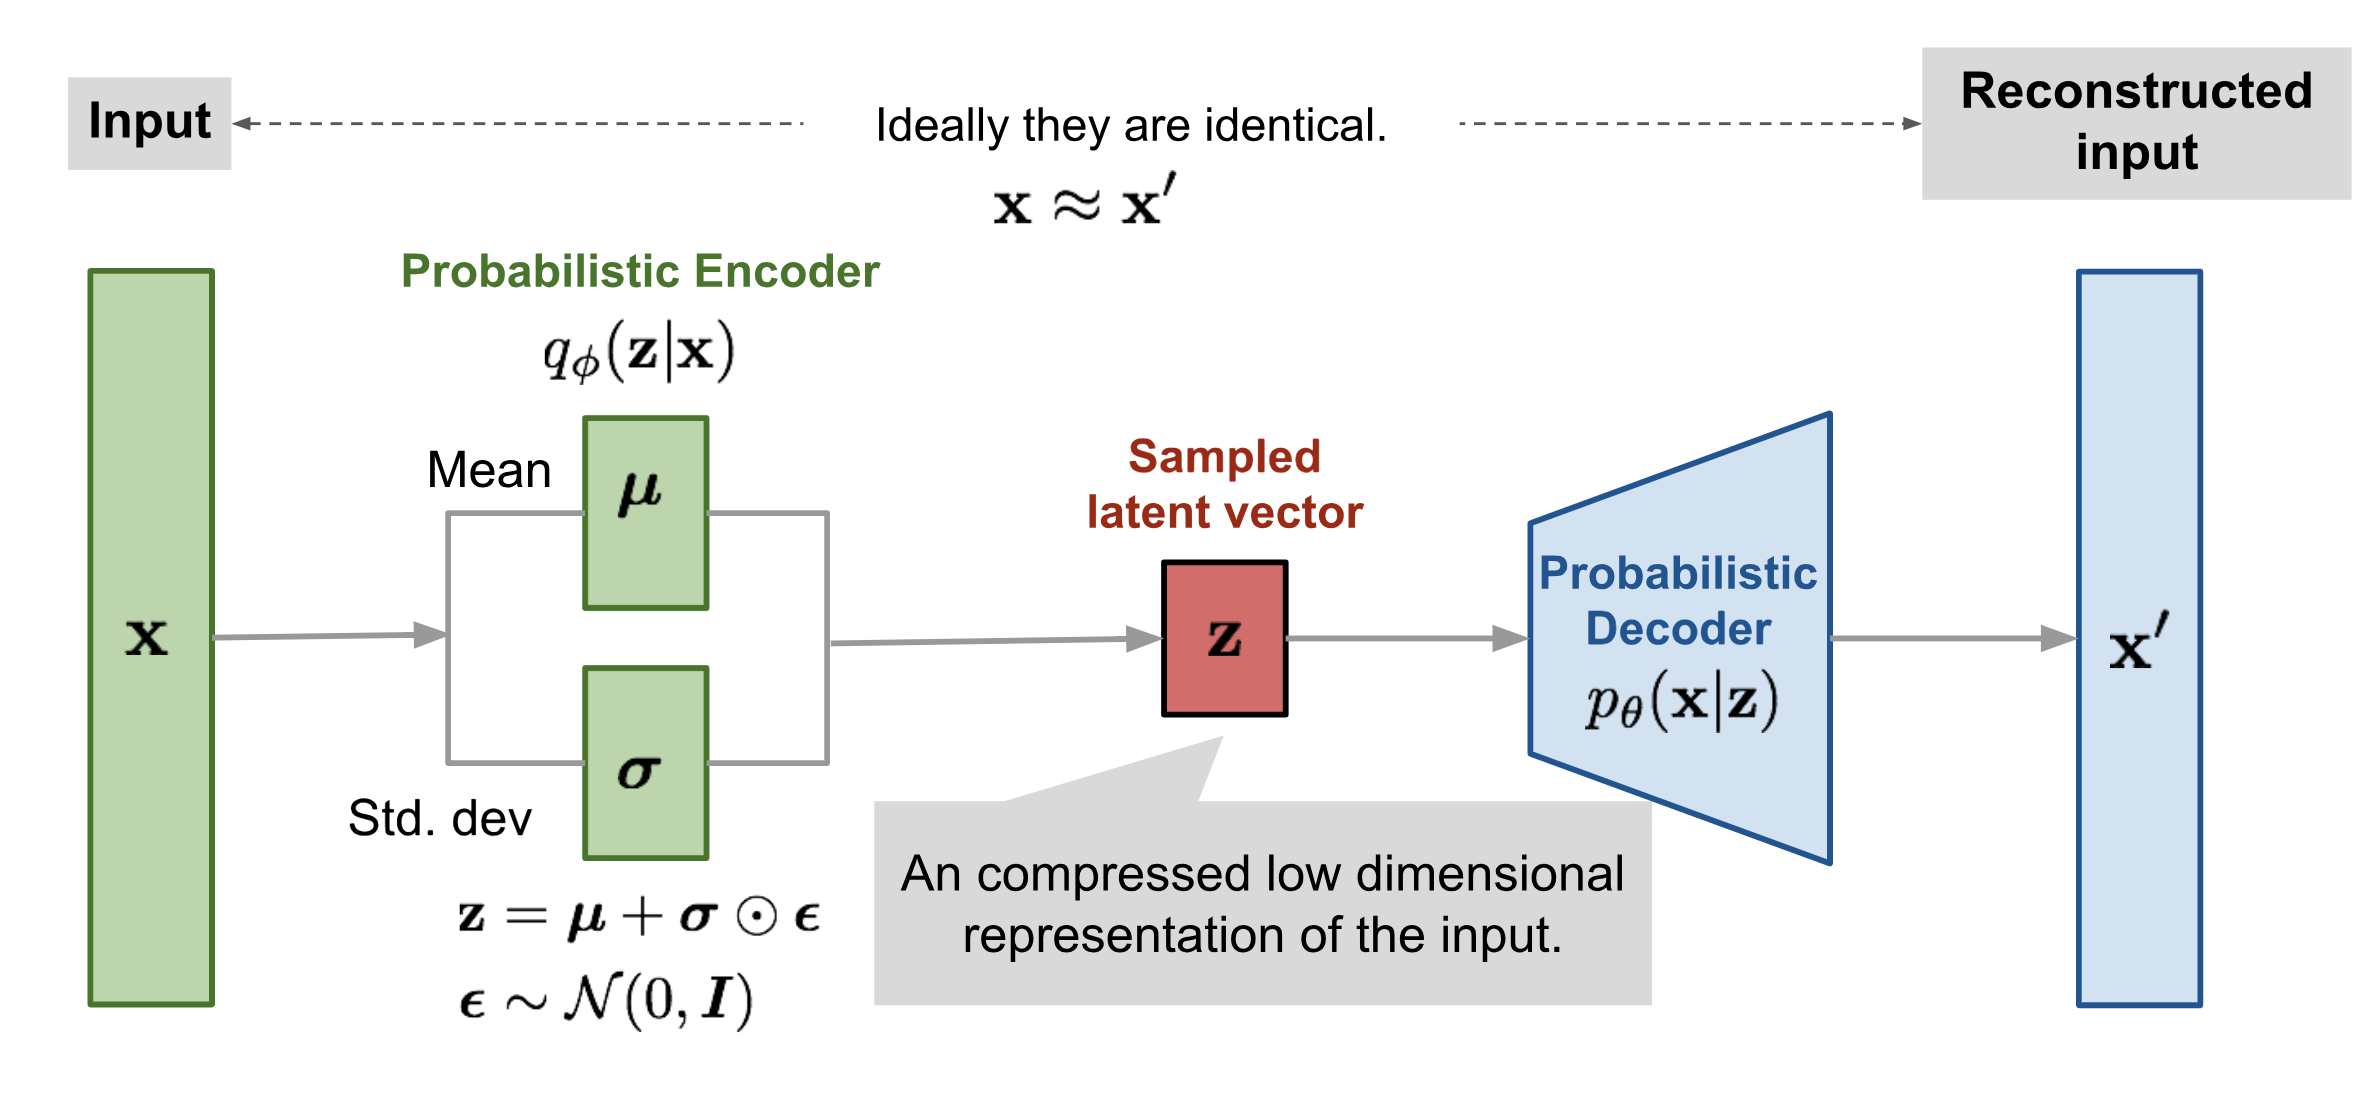
\includegraphics[width=0.8\textwidth]{vae}
\end{center}

\end{frame}

\begin{frame}{Generative models: adversarial networks}

\begin{center}
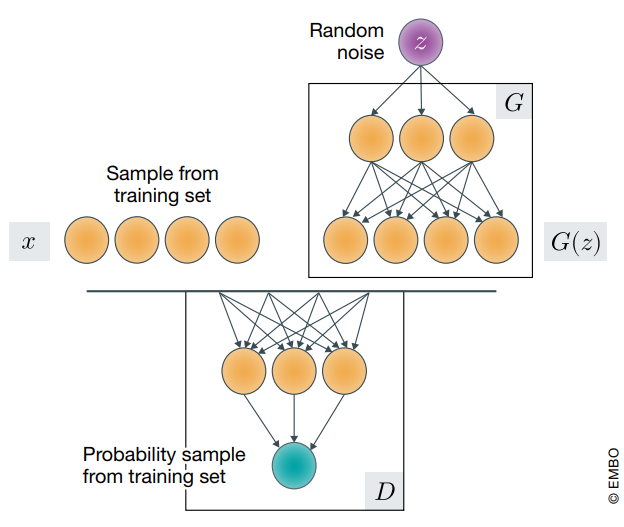
\includegraphics[width=0.8\textwidth]{gan}
\end{center}


\end{frame}

\begin{frame}{Cool biological applications of VAEs and GANs}

Sequencing, Imaging, Other stuff

\end{frame}


\begin{frame}{Monte-Carlo Markov Chain (MCMC)}

\begin{itemize}

\item MCMC algorithms were originally developed in the 1940’s by physicists at
Los Alamos

\item They were interested in modeling the probabilistic behavior of collections of
atomic particles

\item Simulation was difficult – the normalization constant $Z$ was not known

\item The term “Monte-Carlo” was coined at Los Alamos.

\item Ulam and Metropolis overcame this problem by constructing a Markov chain
for which the desired distribution was the stationary distribution

\item Introduced to statistics and generalized with the Metropolis-Hastings
algorithm (1970) and the Gibbs sampler of Geman and Geman (1984).
\end{itemize}

\end{frame}

\begin{frame}{Monte-Carlo Markov Chain (MCMC)}

MCMC is used when we know the functional form of $p(\mathbf{x})$ up to the normalization constant e.g., Ising model\\
\vspace{0.1in}
MCMC methods do not model $p(\mathbf{x})$ directly but allow us to draw samples $\mathbf{x} \sim p(\mathbf{x})$

\end{frame}

\begin{frame}{Gibbs sampling}

\end{frame}


\section{Probabilistic Graphical Models}

\begin{frame}{Probabilistic graphical models}

\end{frame}

\begin{frame}{Using Gibbs sampling with graphical models}

\end{frame}

\section{References}

% Adding the option 'allowframebreaks' allows the contents of the slide to be expanded in more than one slide.
\begin{frame}[allowframebreaks]{References}
	\tiny\bibliography{references}
	\bibliographystyle{apalike}
\end{frame}

\end{document}